%initialising document, adjust papersize, fontsize and page orientation to your needs
\documentclass[a4paper, fontsize = 8pt, landscape]{scrartcl}
\usepackage{layout_and_colours}
\title{Theoretische Informatik}
\author{Lucien Perret, Jil Zerndt}
\date{May 2024}

\createtitlepagestyle
\createmainpagestyle

\begin{document}
\begin{multicols*}{3}
    \thispagestyle{TitlePageStyle}
		\maketitle

    \input{1_Alphabete_Wörter_Sprachen.tex}
    \raggedcolumns
    \begin{definition}{Reguläre Ausdrücke}
    Wörter, die Sprachen beschreiben (Regex)
\end{definition}

\begin{concept}{$R A_{\Sigma}$}
    Sprache der Regulären Ausdrücke über $\{\emptyset, \epsilon, *,(),, \mid\} \cup \Sigma$ 
    
    \begin{minipage}{0.69\linewidth}
    \begin{itemize}
        \item $R, S \in R A_{\Sigma}$ $\Rightarrow(R^{*}), (R S), (R \mid S) \in R A_{\Sigma}$  
    \end{itemize}
    \end{minipage}
    \begin{minipage}{0.3\linewidth}
        \begin{itemize}
            \item $\emptyset, \epsilon, \Sigma \in R A_{\Sigma}$
        \end{itemize}
    \end{minipage}

    \vspace*{1mm}

    \textbf{Priorisierung von Operatoren}
    
    (1) $*=$ Wiederholung $\rightarrow$ (2) Konkatenation $\rightarrow$ (3) $\mid=$ Oder
    
    \textbf{Erweiterter Syntax}

        $
        \begin{array}{lcr}
            R^{+} = R (R^{*}) & R ?=(R \mid \epsilon) & \quad \left[R_{1}, \ldots, R_{k}\right]=R_{1}\left|R_{2}\right| \ldots \mid R_{k} 
        \end{array}
        $
\end{concept}



\begin{definition}{Reguläre Sprache}
    $A$ über dem Alphabet $\Sigma$ heisst regulär, falls \textcolor{pink}{$A=L(R)$} für einen regulären Ausdruck $R \in R A_{\Sigma}$ gilt.
\end{definition} 

\begin{concept}
    {$\forall  R \in R A_{\Sigma}$} definieren wir die Sprache $L(R)$ von $R$ wie folgt:\\
    \begin{minipage}{0.4\linewidth}
        \begin{itemize}
            \item $L(\emptyset)=\emptyset$
            \item $L(\varepsilon)=\{\varepsilon\}$
            \item $L(a)=\{a\} \quad \forall a \in \Sigma$
            \item $L(R^{*})=L(R)^{*}$
            \item $L((R^{*})^{*})=L(R^{*})$
            \item $L(R S) = L(R)L(S)$
            
        \end{itemize}
    \end{minipage}
    \begin{minipage}{0.55\linewidth}
        \begin{itemize}
            \item $L(R \mid S) = L(S \mid R)$
            \item $L(R(ST))=L((RS)T)=L(R S)$
            \item $L(R \mid (S \mid T))=L((R \mid S) \mid T)$
            \item $L(R(S \mid T))= L(RS \mid RT)$
            \item $L(R \mid R)=L(R)=L(R \mid \emptyset)$
            \item $L(R \mid S)=L(R) \cup L(S)$
        \end{itemize}
    \end{minipage}
\end{concept}









    \raggedcolumns
    \section*{Endliche Automaten}

\begin{definition}{Endliche Automaten}
    Maschinen, die Entscheidungsprobleme lösen\\
    \begin{minipage}{0.35\linewidth}
        \begin{itemize}
            \item Links nach rechts
            \item Keinen Speicher
            \item Keine Variablen
        \end{itemize}
    \end{minipage}
    \begin{minipage}{0.5\linewidth}
        \begin{itemize}
            \item Speichert aktuellen Zustand
            \item Ausgabe über akzeptierende Zustände
        \end{itemize}
    \end{minipage}
\end{definition}

\begin{definition}{DEA} deterministischer endlicher Automat: $M=(Q, \Sigma, \delta, q_{0}, F)$
    \begin{itemize}
    \item $Q$ endliche Menge von Zuständen
    \item $\Sigma$ endliches Eingabealphabet
    \item $\delta: Q \times \Sigma \rightarrow Q$ Übergangsfunktion
    \item $q_{0} \in Q$ Startzustand
    \item $F \subseteq Q$ Menge der akzeptierenden Zustände
    \end{itemize}
\end{definition}

\begin{KR}{DEA Funktionen}
    $M=\left(Q, \Sigma, \delta, q_{0}, F\right)$ : EA.\\ \textbf{Konfiguration} von $M$ auf $\omega$ ist ein Element aus $Q \times \Sigma^{*}$
    \begin{itemize}
    \item Startkonfiguration von $M$ auf $\omega \quad \left\{q_{0}, \omega\right\} \in\left\{q_{0}\right\} \times \Sigma^{*}$
    \item Endkonfiguration $\quad \left(q_{n}, \varepsilon\right)$
    \end{itemize}

    \textbf{Berechnungsschritt} $\vdash_{M}$ von $M$
    $
    (q, \omega) \vdash_{M}(p, x)
    $

    \textbf{Berechnung} ist eine endliche Folge von Berechnungsschritten
    \resizebox{\linewidth}{!}{
    $
    \left(q_{a}, \omega_{1} \omega_{2} \ldots \omega_{n}\right) \vdash_{M} \ldots \vdash_{M}\left(q_{e}, \omega_{j} \ldots \omega_{n}\right) \rightarrow\left(q_{a}, \omega_{1} \omega_{2} \ldots \omega_{n}\right) \vdash_{M}^{*}\left(q_{e}, \omega_{j} \ldots \omega_{n}\right)
    $
    }
\end{KR}

\begin{example2}{Beispiel DEA (eindeutig)} Sprache: $L(M)=\left\{1 x 1 \mid x \in\{0\}^{*}\right\}$
    
    \begin{minipage}{0.45\linewidth}
        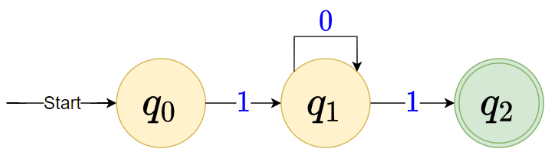
\includegraphics[width=1\linewidth]{images/dea_example.png}
    \end{minipage}
    \hspace{1mm}
    \begin{minipage}{0.5\linewidth}
        \textbf{Konfiguration} auf $\omega=101$
        \begin{itemize}
        \item Startkonfiguration $\rightarrow\left(q_{0}, 101\right)$
        \item Endkonfiguration $\rightarrow\left(q_{2}, \varepsilon\right)$
        \end{itemize}
    \end{minipage}

    \textbf{Berechnung}

    \resizebox{\linewidth}{!}{
    $\omega=101 \rightarrow\left(q_{0}, 101\right) \vdash_{M}\left(q_{1}, 01\right) \vdash_{M}\left(q_{1}, 1\right) \vdash_{M}\left(q_{2}, \varepsilon\right) \rightarrow \text{akzeptierend}$\\
    }

    \resizebox{\linewidth}{!}{
    $\omega=10 \rightarrow\left(q_{0}, 10\right) \vdash_{M}\left(q_{1}, 0\right) \vdash_{M}\left(q_{1}, \varepsilon\right) \rightarrow \text{verwerfend}$
    }
\end{example2}

\begin{definition}{Nichtdeterministischer endlicher Automat (NEA)}\\
    \begin{minipage}{0.75\linewidth}
        Unterschied zum DEA: Übergangsfunktion $\delta$\\
        Übergangsfunktion $\delta: Q \times \Sigma \rightarrow P(Q)$\\
        Ein $\varepsilon$-NEA erlaubt zusätzlich noch $\varepsilon$-Übergänge
    \end{minipage}  
    \begin{minipage}{0.2\linewidth}
        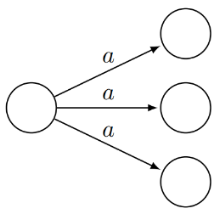
\includegraphics[width=1\linewidth]{images/ndea.png}
    \end{minipage}
\end{definition}

\begin{example2}{NEA (nicht eindeutig)} Sprache: $L(M)=\left\{x 01 \mid x \in\{0,1\}^{*}\right\}$
    
    \begin{minipage}{0.55\linewidth}
        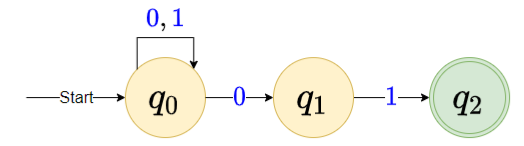
\includegraphics[width=1\linewidth]{images/nea_example1.png}
    \end{minipage}
    \hspace{1mm}
    \begin{minipage}{0.4\linewidth}
        \includegraphics[width=1\linewidth]{images/äquivalenter_nea.png}
        
        äquivalenter DEA
    \end{minipage}    
\end{example2}

\begin{formula}{Teilmengenkonstruktion}
    $\forall$ NEA kann in DEA umgewandelt werden
    \begin{enumerate}
        \item $Q_{N E A} \rightarrow P\left(Q_{N E A}\right)=Q_{D E A} \quad$ (Potenzmenge)
        \item Verbinden mit Vereinigung aller möglichen Zielzustände
        \item Nicht erreichbare Zustände eliminieren
        \item Enthält akzeptierenden Zustand $=F_{N E A} \rightarrow$ akzeptierend
    \end{enumerate}

    \begin{minipage}{0.5\linewidth}
        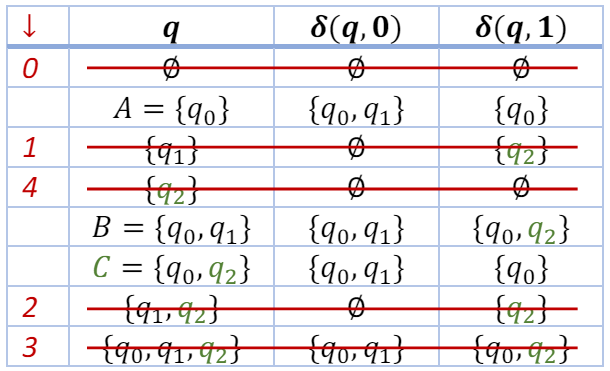
\includegraphics[width=1\linewidth]{images/teilmengenkonstruktion.png}
    \end{minipage}
    \begin{minipage}{0.5\linewidth}
        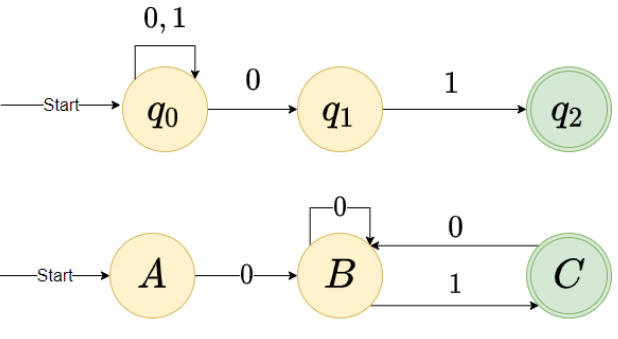
\includegraphics[width=1\linewidth]{images/teilmengenkonstruktion2.png}
    \end{minipage}
\end{formula}    
    \raggedcolumns
    \input{4_Reguläre_Sprachen.tex}
    \raggedcolumns
    \graphicspath{{images/}}
\section*{Kontextfreie Grammatiken}

\begin{definition}{Kontextfreie Grammatik} $(K F G)$ ist ein 4-Tupel $(N, \Sigma, P, A)$ mit
    \begin{itemize}
    \item $N$: Alphabet der Nichtterminale (Variablen)
    \item $\Sigma$: Alphabet der Terminale
    \item $P$: endliche Menge von Produktionen mit der Form $X \rightarrow \beta$
    \end{itemize}

    $\quad$ Mit Kopf $X \in N$ und Rumpf $\beta \in(N \cup \Sigma)^{*}$

    \begin{itemize}
    \item $A$: Startsymbol, wobei $A \in N$
    \end{itemize}

    Ein Wort $\beta \in(N \cup \Sigma)^{*}$ nennen wir Satzform.

    Seien $\alpha, \beta$ und $\gamma$ Satzformen und $A \rightarrow \gamma$ eine Produktion.

    \begin{itemize}
    \item Ableitungsschritt mit Produktion $A \rightarrow \gamma \quad \alpha A \beta \rightarrow \alpha \gamma \beta$
    \item Ableitung Folge von Ableitungsschritten $\alpha \rightarrow \cdots \rightarrow \omega$
    \end{itemize}
\end{definition}

\begin{definition}{Ableitungsbaum (Parsebaum)} mögliche Darstellung einer Ableitung

    \begin{itemize}
    \item $G_{1}=\{\{A, B, C\},\{0,1\}, P, A\}$
    \item $P=\{A \rightarrow B C, B \rightarrow 0 B|0| \varepsilon, C \rightarrow 1 C|1| \varepsilon\}$
    \end{itemize}

    Ableitung von $\omega_{1}=011$

    \begin{itemize}
    \item $A \rightarrow B C \rightarrow 0 A A \rightarrow 01 C \rightarrow 011 \rightarrow \ldots \rightarrow 011$
    \end{itemize}
    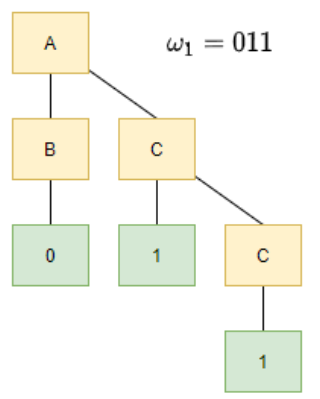
\includegraphics[width=0.3\linewidth]{ableitungsbaum.png}
\end{definition}

\begin{concept}{Mehrdeutigkeit}\\
    Eine KFG nennen wir mehrdeutig, wenn es ein Wort gibt, das mehrere Ableitungsbäume besitzt.\\
    \textbf{Mehrdeutigkeiten eliminieren:}
    \begin{itemize}
    \item Korrekte Klammerung vom Benutzer erzwingen
    \item Grammatik anpassen
    \item Den Produktionen einen Vorrang vergeben
    \end{itemize}
\end{concept}

\begin{KR}{KFG für Sprache L}\\
    Jede reguläre Sprache kann durch eine kontextfreie Grammatik beschrieben werden. Sei $L$ eine reguläre Sprache. Dann gibt es einen DEA $M=\left(Q, \Sigma, \delta, q_{0}, F\right)$ mit $L(M)=L$\\
    Dann können wir einen KFG für $L$ wie folgt bauen:
    \begin{itemize}
    \item Für jeden Zustand $q_{i}$ gibt es ein Nichtterminal $Q_{i}$
    \item Für jede Transition $\delta\left(q_{i}, a\right)=q_{j}$ erstellen wir die Produktion $Q_{i} \rightarrow a Q_{j}$
    \item Für jeden akzeptierenden Zustand $q_{i} \in F$ erstellen wir die Produktion $Q_{i} \rightarrow \varepsilon$
    \item Das Nichtterminal $Q_{0}$ wird zum Startsymbol $A$.
    \end{itemize}
\end{KR}
    \raggedcolumns
    \graphicspath{{images/}}
\section*{Kellerautomaten}

\begin{remark}
    KA auf englisch: PDA = Push Down Automat
\end{remark}

\begin{definition}{Kellerautomaten}(KA) besitzt «Speicher»

    Deterministischer KA (DKA): $M=\left(Q, \Sigma, \boldsymbol{\Gamma}, \boldsymbol{\delta}, q_{0}, \$, F\right)$
    
    \begin{minipage}{0.4\linewidth}
        $Q$: Menge von Zuständen

        $\Sigma$: Alphabet der Eingabe

        $\Gamma$: Alphabet des Kellers
    \end{minipage}
    \begin{minipage}{0.6\linewidth}
        $q_{0} \in Q$: Anfangszustand

        $\$ \in \Gamma$: Symbol vom Alphabet des Kellers

        $F \subseteq Q$: Akzeptierende Zustände
    \end{minipage}

    Übergangsfunktion: $\boldsymbol{\delta}: \boldsymbol{Q} \times(\boldsymbol{\Sigma} \cup \boldsymbol{\varepsilon}) \times \boldsymbol{\Gamma} \rightarrow \boldsymbol{Q} \times \Gamma^{*}$

    \vspace{1mm}

    \textcolor{pink}{NKA:} $\delta: Q \times(\Sigma \cup \varepsilon) \times \Gamma \rightarrow P(Q \times \Gamma *)$ (Nichtdeterministischer KA)
\end{definition}

\begin{concept}{Übergangsfunktion KA}
    $\forall$ Zustand $q$ und $\forall$ Symbole $x, b$ gilt:
    
    wenn $\delta(q, b, c)$ definiert ist, dann ist $\delta(q, \varepsilon, x)$ undefiniert.

    \vspace*{1mm}

    Darstellung Übergang $\delta(q, b, c)=(p, \omega)$: \emph{$\quad q -b, c / \omega \longrightarrow p$}
\end{concept}

\begin{formula}{Berechnungsschritt}$\delta(q, b, c)=(p, \omega)$ wird wie folgt interpretiert:
    
    \begin{minipage}{0.45\linewidth}
            $q=$ Aktueller Zustand

            $b=$ gelesene Eingabe

            $c=$ entfernt von Stack (pop)
    \end{minipage}
    \begin{minipage}{0.55\linewidth}
            $\omega=$ aktueller Stack + $\omega$ (push)
            \\neustes Symbol zuerst

            $p=$ Neuer Zustand
    \end{minipage}

    {\small (q, b, c) wird als Konfiguration bezeichnet}
\end{formula}

\begin{definition}{Sprache $L(M)$} eines Kellerautomaten $M$ ist definiert durch

    \resizebox{\linewidth}{!}{
    $
    L(M)=\left\{\omega \in \Sigma^{*} \mid\left(q_{0}, \omega, \$\right) \vdash^{*}(q, \varepsilon, \gamma) \text { für ein } q \in F \text { und ein } \gamma \in \Gamma^{*}\right\}
    $
    }
    Elemente von $L(M)$ werden von $M$ akzeptierte Wörter genannt.
\end{definition}

\begin{remark}
    Damit $w_x$ akzeptiert wird, muss $b = \varepsilon$ sein (Stack muss nicht leer sein)
\end{remark}

\begin{KR}{Kellerautomat für kontextfreie Sprache} $\left\{0^{n} 1^{n} \mid n>0\right\}$
    
    \begin{minipage}{0.5\linewidth}
        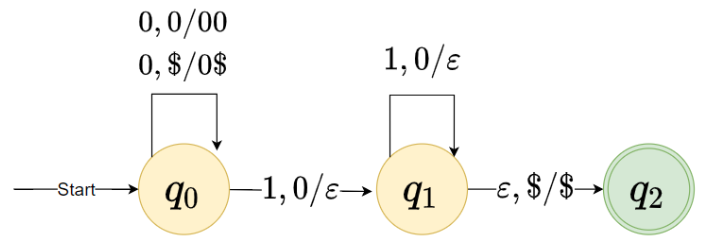
\includegraphics[width=1\linewidth]{kellerautomat_sprache.png}
    \end{minipage}
    \begin{minipage}{0.5\linewidth}
        $\omega_{1}=011:$

        \resizebox{\linewidth}{!}{
        $(q_{0}, 011, \$) \vdash(q_{1}, 11,0 \$) \vdash(q_{1}, 1, \$)$}
        $\rightarrow \omega_{1}$ verwerfend 
        
        Das Zeichen \$ zeigt an, dass der «Stack» leer ist.
    \end{minipage}
\end{KR}

\begin{remark}
    Eine Sprache ist kontextfrei, wenn sie von einem NKA akzeptiert wird (nicht unbedingt von DKA).
    Wenn von DKA erkannt, dann ist die Sprache eindeutig.
\end{remark}

\begin{minipage}{0.4\linewidth}
    \begin{concept}{NKA}$\{\omega \omega^{R} \mid \omega \in\{0,1\}^{*}\}$
    \end{concept}
\end{minipage}
\begin{minipage}{0.6\linewidth}
        \includegraphics[width=1\linewidth]{nka_übergangsfunktion.png}
\end{minipage}


\begin{example2}{NKA/DKA erkennbar?}
    $L_1 = \{0^n1^n0^n \mid n \in \N\}$, $\sigma = \{0,1\} \rightarrow$ nein

    $L_2 = \{waw^R \mid w \in \{0,1\}^*\}$, $\sigma = \{0,1,a\} \rightarrow$ ja (DKA)

    $L_3 = \{ww \mid w \in \{0,1\}^*\}$, $\sigma = \{0,1\} \rightarrow$ nein
\end{example2}


    \raggedcolumns
    \graphicspath{{images/}}

\section*{Turingmaschinen}

\begin{theorem}{Turingmaschinen (TM)}
    \begin{itemize}
        \item Einen Lese- / Schreib-Kopf
        \item Ein unendliches Band von Zellen
      \end{itemize}
      
      Eine deterministischer Turing-Maschine TM ist ein 7-Tupel
      $$
      M=\left(Q, \Sigma, \Gamma, \delta, q_{0}, \sqcup , F\right)
      $$
      \begin{itemize}
        \item Menge von Zuständen: $Q$
        \item Alphabet der Eingabe: $\Sigma$
        \item Bandalphabet: $\Gamma$ und $\Sigma \subset \Gamma$
        \item Übergangsfunktion: $\boldsymbol{\delta}: \boldsymbol{Q} \times \boldsymbol{\Gamma} \rightarrow \boldsymbol{Q} \times \boldsymbol{\Gamma} \times \boldsymbol{D}, \boldsymbol{D}=\{\boldsymbol{L}, \boldsymbol{R}\}$
        \item Anfangszustand: $q_{0} \in Q$
        \item Akzeptierende Zustände: $F \subseteq Q$
        \item Leerzeichen ${ }_{\sqcup }$, mit ${ }_{\mu} \in \Gamma$ und ${ }_{\mu} \notin \Sigma$
      \end{itemize}
      Sie bildet das 2-Tupel $(q, X)$ auf das Tripel $(p, Y, D)$

    \begin{itemize}
    \item $q, p \in Q$ und $X, Y \in \Gamma$
    \item $D=$ Direction
    \item $X=$ Read
    \item $Y=$ Overwrite
    \end{itemize}
    $$
    q-X / Y, D \rightarrow p
    $$
\end{theorem}

\begin{definition}{Band}
    \begin{itemize}
        \item Unterteilt in einzelne Zellen mit jeweils einem beliebigen Symbol
        \item Beinhaltet zu Beginn die Eingabe, d.h. ein endliches Wort aus $\Sigma^{*}$. Alle anderen Zellen enthalten das besondere Symbol 4 .
    \end{itemize}
\end{definition}

\begin{definition}{Konfiguration}
    einer Turing-Maschine $M$ ist durch die folgenden Angaben eindeutig spezifiziert
    \begin{itemize}
    \item Zustand der Zustandssteuerung
    \item Position des Lese- / Schreibkopfes
    \item Bandinhalt
    \end{itemize}
\end{definition}

\begin{concept}{Semi-Unendliches Band}\\
    Das Band der Turingmaschine ist nur in eine Richtung unendlich.\\
    Jede Sprache $L$ die von einer TM $T$ akzeptiert wird, wird auch von einer TM mit semi-unendlichem Band akzeptiert.\\
    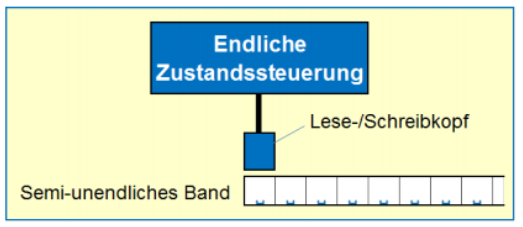
\includegraphics[width=0.3\linewidth]{semi_unendliches_band.png}
\end{concept}

\begin{concept}{Mehrere Stacks}\\
    Jede Sprache $L$ die von einer TM $T$ akzeptiert wird, wird auch von einer 2Stack-Maschine $S$ akzeptiert.\\
    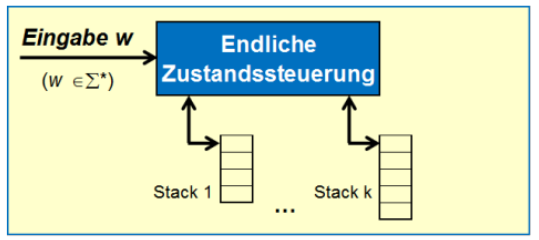
\includegraphics[width=0.3\linewidth]{mehrere_stacks_tm.png}
\end{concept}

\begin{concept}{Zähler-Maschinen}\\
    Eine Zähler-Maschine (Counter Machine) mit $k$ Zählern entspricht einer $k$ Stack-Maschine mit dem Unterschied, dass die Stacks durch einfache Zähler ersetzt werden.\\
    Jede Sprache $L$ die von einer TM $T$ akzeptiert wird, wird auch von einer 2Zähler-Maschine $Z$ mit 2 Zählern akzeptiert.\\
    \includegraphics[width=0.3\linewidth]{zähler_maschinen.png}
\end{concept}

\begin{concept}{TM mit Speicher}\\
    In der endlichen Zustandssteuerung einer TM können ausser dem SteuerZustand zusätzlich endlich viele Daten-Zustände gespeichert werden.\\
    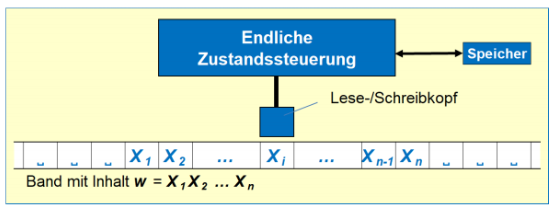
\includegraphics[width=0.3\linewidth]{tm_mit_speicher.png}
\end{concept}

\begin{concept}{Mehrere Spuren}
    \begin{itemize}
        \item Das Band der TM setzt sich aus mehreren «Spuren» zusammen.
        \item Jede Spur kann ein Symbol des Bandalphabets speichern.
    \end{itemize}
    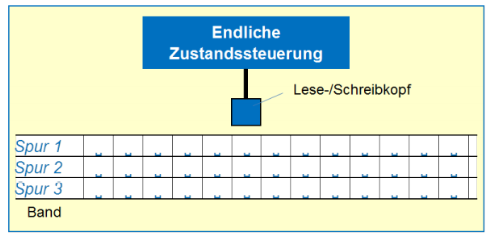
\includegraphics[width=0.3\linewidth]{mehrere_spuren.png}
\end{concept}

\begin{concept}{Mehrere Bänder}
    \begin{itemize}
        \item TM mit endlich vielen Bändern und Lese- / Schreibköpfen
        \item Jeder Lese- / Schreibkopf kann unabhängig auf ein Band zugreifen
    \end{itemize}
    \includegraphics[width=0.3\linewidth]{mehrere_bänder.png}
\end{concept}

\begin{example2}{Mehrband-Maschine}\\
    Spezifizieren Sie eine TM $M_{4}$, welche die Subtraktion von zwei natürlichen Zahlen $(a-b$, mit $a \geq b)$ realisiert.\\
    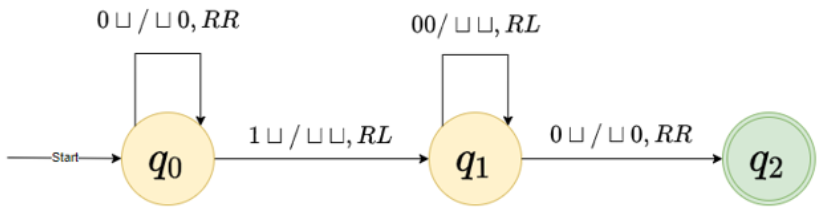
\includegraphics[width=0.5\linewidth]{mehrband_maschine1.png}\\
    Beispiel: $4-2=2$\\
    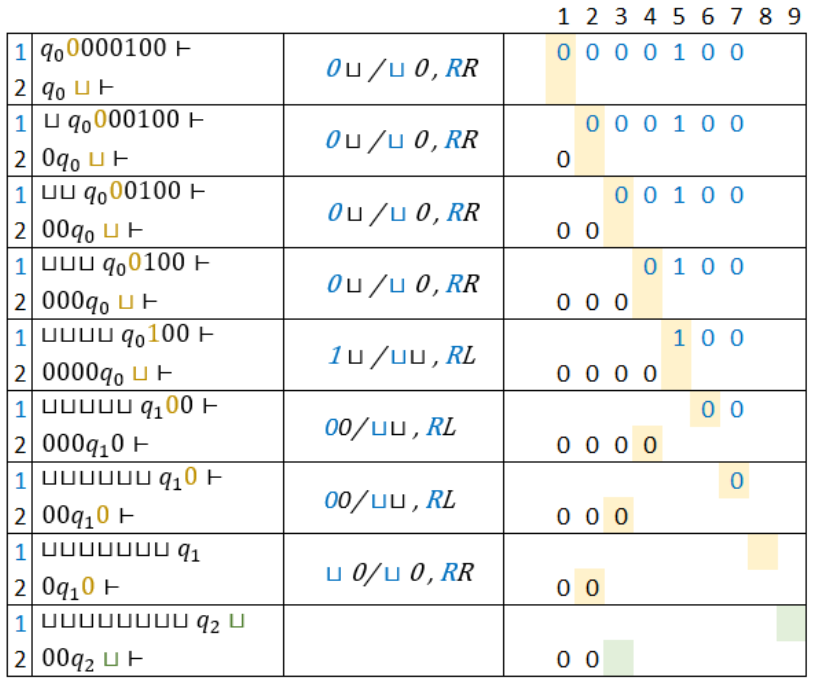
\includegraphics[width=1\linewidth]{mehrband_maschine2.png}
\end{example2}
    \raggedcolumns
    \graphicspath{{images/}}

\section*{Berechnungsmodelle}

\begin{definition}{Turing-berechenbar} = kann von Turing-Maschine gelöst werden
    
    Turing-berechenbare Funktion $T: \Sigma^* \rightarrow \delta^*$

    $T(\omega) = \begin{cases}
        u & \text{falls T auf } \omega \in \Sigma^* \text{ angesetzt, nach endlich vielen}\\ 
        &\text{Schritten mit u auf dem Band anhält}\\
        \uparrow & \text{falls T bei Input } \omega \in \Sigma^* \text{ nicht hält}
    \end{cases}$
\end{definition}

\begin{remark}
    {\footnotesize
    $\forall$ algorithmisch lösbare Problem ist turing-berechenbar $\Rightarrow$ Computer $\equiv$ TM
    }
\end{remark}

\begin{theorem}{Primitiv rekursive Grundfunktionen} $\forall n \in \mathbb{N}$, $\forall k \in \mathbb{N}$ {\footnotesize (k = Konstante)}
    
    \vspace{1mm}

    n-stellige konstante Funktion: $c_k^n = \mathbb{N}^n \rightarrow \mathbb{N} \text{ mit } c_k^n (x_1, ... , x_n) = k$

    \vspace{1mm}

    Nachfolgerfunktion: $\eta : \mathbb{N} \rightarrow \mathbb{N} \text{ mit } \eta (x) = x + 1$

    \vspace{1mm}
    
    n-stellige Projektion auf die k-te Komponente: 

    \vspace{1mm}

    $\quad \pi_k^n : \mathbb{N}^n \rightarrow \mathbb{N} \text{ mit } \pi_k^n (x_1, ... ,x_k,..., x_n) = k$ {\footnotesize $\quad$ ($1 < k < n$)}
    
    {\small n = Anzahl der Argumente, k = Position des Arguments}
\end{theorem}

\begin{minipage}
    {0.62\linewidth}
\begin{concept}{LOOP{,} WHILE{,} GOTO}

        Zuweisung: $xi = xj + c$ oder $xi = xj - c$\\
        Nach Ablauf eines Programms steht der Wert der Berechnung in der Variable $x_0$
\end{concept}
\end{minipage}
\begin{minipage}{0.34\linewidth}
    {\small
    Variablen: $x0, x1, x2, ...$\\
Konstanten: $0, 1, 2, ...$\\
Operationszeichen: $+, -$\\
Trennzeichen: $;$}
\end{minipage}

\begin{minipage}{0.5\linewidth}
    \begin{KR}{Loop (primitiv-rekursiv)}

            Schlüsselwörter: Loop, Do, End

            Sequenzen: $P$ und $Q \rightarrow P; Q$

            Schleifen: Loop $x$ do $P$ ... End
    \end{KR}
    \end{minipage}
    \begin{minipage}{0.5\linewidth}
    \begin{example}    
\begin{lstlisting}[style=Pseudocode, aboveskip=-0.5\baselineskip, belowskip=-0.5\baselineskip]
Loop x1 Do
    x2 = x2 + 1
End;
x0 = x2 + 0
\end{lstlisting}
    \end{example}
\end{minipage}

\begin{minipage}{0.5\linewidth}
    \begin{KR}{While (Turing vollständig)}

        Erweiterung der Sprache Loop

        While $xi > 0$ Do ... End
    \end{KR}
    \begin{example}        
\begin{lstlisting}[style=Pseudocode, aboveskip=-0.5\baselineskip, belowskip=-0.5\baselineskip]
While x1 > 0 Do
    x1 = x1 - 1;
    Loop x2 Do
        x0 = x0 + 1
    End
End
\end{lstlisting}
\end{example}
\end{minipage}
\begin{minipage}{0.5\linewidth}
\begin{KR}{GoTo (Turing vollständig)}\\
        Schlüsselwörter: Goto, If, Else
        
        Marker Mk: M1, M2, ...
        
        Sprunganweisung:\\ If $xi = c$ Then Goto $Mk$ 
\end{KR}
\begin{example}
\begin{lstlisting}[style=Pseudocode, aboveskip=-0.5\baselineskip, belowskip=-0.5\baselineskip]
M1: x0 = x3 + 0;
M2: If x1 = 0 Then Goto M4;
M3: x0 = x2 + 0;
M4: Halt
\end{lstlisting}
\end{example}
\end{minipage}

    \raggedcolumns
    \columnbreak
    \graphicspath{{images/}}

\section*{Entscheidbarkeit}

\begin{theorem}{Entscheidbarkeit}\\
    \begin{itemize}
        \item Ein Problem ist entscheidbar, wenn es einen Algorithmus gibt, der für jede Eingabe eine Antwort liefert.
        \item Ein Problem ist semi-entscheidbar, wenn es einen Algorithmus gibt, der für jede Eingabe eine Antwort liefert, falls die Antwort ja ist.
    \end{itemize}
    Eine Sprache $A \subset \Sigma^{*}$ ist genau dann entscheidbar, wenn sowohl $A$ als auch $\bar{A}$ semi-entscheidbar ist.
    \begin{itemize}
        \item $\bar{A}$ steht für das Komplement von $A$ in $\Sigma^{*}: \quad \bar{A}=\Sigma^{*} \backslash A=\left\{\omega \in \Sigma^{*} \mid \omega \notin A\right\}$
    \end{itemize}
\end{theorem}

\begin{corollary}{Entscheidbarkeit und Turingmaschinen}
    Eine Sprache $A \subset \Sigma^{*}$ heisst entscheidbar, wenn eine TM $T$ existiert, die sich wie folgt verhält:
    \begin{itemize}
    \item Bandinhalt $x \in A \quad T$ hält mit Bandinhalt «1» (Ja) an
    \item Bandinhalt $x \in \Sigma^{*} \backslash A \quad T$ hält mit Bandinhalt «0» (Nein) an
    \end{itemize}

    Äquivalente Aussagen:
    \begin{itemize}
        \item $A \subset \Sigma^{*}$ ist entscheidbar
        \item Es existiert eine $T M$, die das Entscheidungsproblem $T(\Sigma, A)$ löst
        \item Es existiert ein WHILE-Programm, dass bei einem zu $A$ gehörenden Wort stets terminiert $\rightarrow$ Entscheidungsverfahren für $A$
    \end{itemize}
\end{corollary}

\begin{corollary}{Semi-Entscheidbarkeit Turingmaschinen}\\
    Eine Sprache $A \subset \Sigma^{*}$ heisst semi-entscheidbar, wenn eine TM $T$ existiert, die sich wie folgt verhält:

    \begin{itemize}
    \item Bandinhalt $x \in A \quad T$ hält mit Bandinhalt «1» (Ja) an
    \item Bandinhalt $x \in \Sigma^{*} \backslash A \quad T$ hält nie an
    \end{itemize}

    Äquivalente Aussagen
    \begin{itemize}
    \item $A \subset \Sigma^{*}$ ist semi-entscheidbar
    \item $A \subset \Sigma^{*}$ ist rekursiv aufzählbar
    \item Es gibt eine TM, die zum Entscheidungsproblem $T(\Sigma, A)$ nur die positiven («Ja») Antworten liefert und sonst gar keine Antwort
    \item Es gibt ein WHILE-Programm, dass bei einem zu $A$ gehörenden Wort stets terminiert und bei Eingabe von Wörtern die nicht zu $A$ gehören nicht terminiert
    \end{itemize}
\end{corollary}

\begin{theorem}{Reduzierbarkeit}\\
    Eine Sprache $A \subset \Sigma^{*}$ heisst auf eine Sprache $B \subset \Gamma^{*}$ reduzierbar, wenn es eine totale, Turing-berechenbare Funktion $F: \Sigma^{*} \rightarrow \Gamma^{*}$ gibt, so dass für alle $\omega \in \Sigma^{*}$
    $$
    \omega \in A \Leftrightarrow F(\omega) \in B
    $$
    \begin{itemize}
    \item $A \preccurlyeq B \quad A$ ist reduzierbar auf $B$
    \item $A \preccurlyeq B$ und $B \preccurlyeq C \rightarrow A \preccurlyeq C$
    \end{itemize}
\end{theorem}

\begin{concept}{Halteproblem}\\
    Das allgemeine Halteproblem $H$ ist die Sprache (\# = Delimiter)
    \begin{itemize}
    \item $\quad H:=\left\{\omega \# x \in\{0,1, \#\}^{*} \mid T_{\omega}\right.$ angesetzt auf $x$ hält $\}$
    \end{itemize}
    Sprachen der Halteprobleme (HP): leeres $H P H_{0}$ und spezielles HP $H_{S}$
    \begin{itemize}
    \item $H_{0}:=\left\{\omega \in\{0,1\}^{*} \mid T_{\omega}\right.$ angesetzt auf das leere Band hält $\}$
    \item $H_{S}:=\left\{\omega \in\{0,1\}^{*} \mid T_{\omega}\right.$ angesetzt auf $\omega$ hält $\}$
    \end{itemize}
    $H_{0}, H_{S}$ und $H$ sind semi-entscheidbar.
\end{concept}
    \raggedcolumns
    \columnbreak
    \input{10_Komplexitätstheorie.tex}
    \raggedcolumns

\end{multicols*}
\end{document}
